\documentclass[review]{elsarticle}

\usepackage{lineno,hyperref}
\modulolinenumbers[1]

\journal{Journal of \LaTeX\ Templates}


%%%%%%%%%%%%%%%%%%%%%%%
%% Elsevier bibliography styles
%%%%%%%%%%%%%%%%%%%%%%%
%% To change the style, put a % in front of the second line of the current style and
%% remove the % from the second line of the style you would like to use.
%%%%%%%%%%%%%%%%%%%%%%%

%% Numbered
%\bibliographystyle{model1-num-names}

%% Numbered without titles
%\bibliographystyle{model1a-num-names}

%% Harvard
%\bibliographystyle{model2-names.bst}\biboptions{authoryear}

%% Vancouver numbered
%\usepackage{numcompress}\bibliographystyle{model3-num-names}

%% Vancouver name/year
%\usepackage{numcompress}\bibliographystyle{model4-names}\biboptions{authoryear}


%% AMA style
%\usepackage{numcompress}\bibliographystyle{model6-num-names}

%% `Elsevier LaTeX' style
%\bibliographystyle{elsarticle-num}

%% APA style
% \bibliographystyle{model5-names}\biboptions{authoryear}

%%%%%%%%%%%%%%%%%%%%%%%

\usepackage{subcaption}

\begin{document}

\begin{frontmatter}

\title{Forecasting the black Sigatoka development rate: A machine learning methods comparison 
%\tnoteref{mytitlenote}
}
%\tnotetext[mytitlenote]{Fully documented templates are %available in the elsarticle package on \href{http://%www.ctan.org/tex-archive/macros/latex/contrib/elsarticle}%{CTAN}.}

%% Group authors per affiliation:
\author[afiLuisAlex]{Luis-Alexander Calvo-Valverde\fnref{myfootnote}}
\ead{lualcava.sa@gmail.com}
\fntext[myfootnote]{Corresponding author. (506)70104420}

\author[afiCorbana] {Mauricio Guzm\'an-Quesada}
\author[afiCorbana]{Jos\'e-Antonio Guzm\'an-Alvarez}
\author[afiPablo]{Pablo Alvarado-Moya}

\address[afiLuisAlex]{DOCINADE, Instituto Tecnol\'ogico de Costa Rica, 
Computer Research Center, Multidisciplinar program eScience, 
CNCA/CeNAT, Cartago, Costa Rica}

\address[afiCorbana]{Direcci\'on de Investigaciones, Corporaci\'on Bananera Nacional S.A., Gu\'apiles, Costa Rica}

\address[afiPablo]{DOCINADE, Instituto Tecnol\'ogico de Costa Rica, Cartago, Costa Rica}




\begin{abstract}
Pending.
\end{abstract}

\begin{keyword}
\texttt{Machine learning \sep Black Sigatoka \sep Support vector regression \sep
Banana disease prediction \sep Biological warning system }
\end{keyword}

\end{frontmatter}

\linenumbers

\section{Introduction}
The Black Sigatoka disease caused by the fungus {\it Mycosphaerella fijiensis Morelet} is the major pathological problem of banana and plantain crops in Central America, Panama, Colombia and Ecuador, as in many parts of Africa and Asia \citep{MarinVargas1995}.\\
This disease attacks the plant leaves producing a rapid deterioration of the leaf area, affects the growth and productivity of plants as the ability of photosynthesis decreases, causes a reduction in the quality of the fruit, and promotes premature maturation of bunches, which is the major cause of product losses due to this disease. \figurename $.$\ref{figura1} shows three stages of this disease.\\
Phytopathological studies point out that precipitation, temperature, relative humidity and wind are the main climatic variables that affect the development of this disease \citep{MarinVargas1995}.\\ 	 	 
\begin{figure}[h] 
\begin{subfigure}{.3\textwidth}
  \centering
  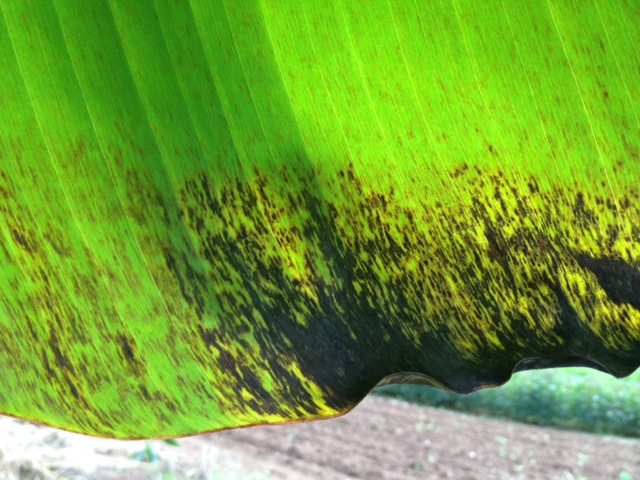
\includegraphics[width=.8\linewidth]{Roya_a}
  \caption{}
  \label{fig:sfig1}
\end{subfigure}
\begin{subfigure}{.3\textwidth}
  \centering
  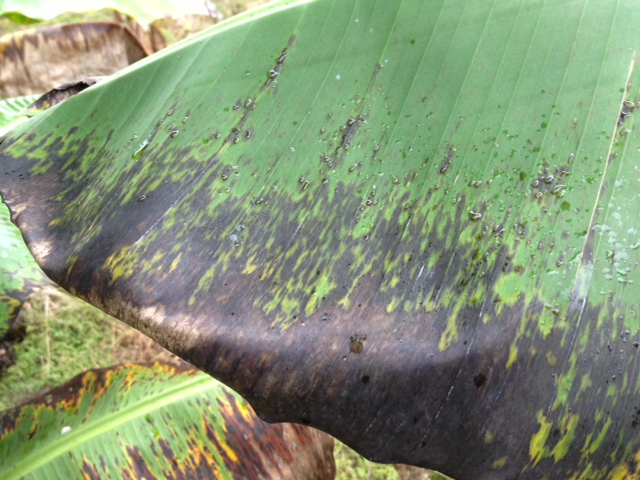
\includegraphics[width=.8\linewidth]{Roya_b}
  \caption{}
  \label{fig:sfig2}
\end{subfigure}
\begin{subfigure}{.3\textwidth}
  \centering
  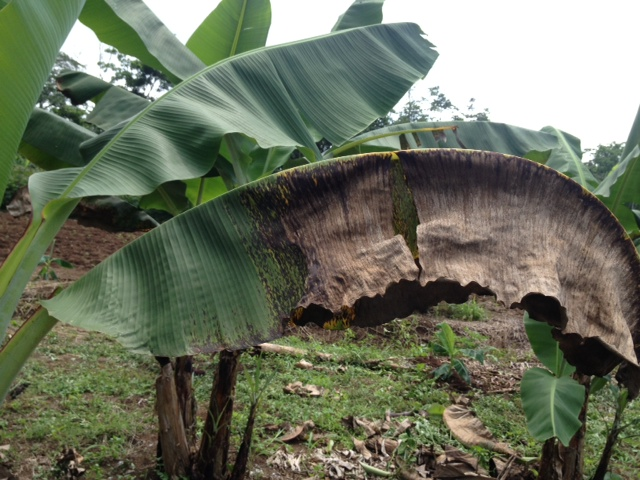
\includegraphics[width=.8\linewidth]{Roya_c}
  \caption{}
  \label{fig:sfig3}
\end{subfigure}
\caption{Examples of three disease stages of the black Sigatoka. (a) Initial stage. (b) Intermediate stage, and (c) Advanced stage.} 
\label{figura1} 
\end{figure}\\
According to studies by the National Banana Corporation of Costa Rica (Corbana) made in 2013, considering on average between 53 thru 57 cycles of fungicide applications per farm, the cost per hectare per year ranged between \$1800 USD and thru \$1900 USD. This represents about 0.76 cents of the price of a box of 18.14 kilograms. Overall, this represents 10\% to 12\% of the total production cost \citet{Bresciani2015}.\\
The past and present disease development rate can in principle be used to predict its future behavior, tendencies and to determine whether particular fungicide spray schedules will be able to effectively and economically control the disease \citet{ChuangJeger1987}.\\
There are efforts to apply machine learning methods for decision-making in agriculture, including the control of crop diseases. For example, \cite{Camargo2012} present an intelligent systems for the assessment of crop disorders, \cite{Huang2010} introduce a plant virus identification method based on neural networks with an evolutionary preprocessing stage, \cite{Kim2014} summarize in their survey crop pests prediction methods using regression and machine learning approaches, while \cite{Zhao2013} present an intelligent agricultural forecasting system based on wireless sensor networks.\\
In this work, we compare four machine learning methods: support vector regression (SVR), echo state networks (ESN), ridge regression, and ordinary least squares linear regression, to predict the black Sigatoka disease development rate.\\
The main contribution of this work is a comparison between machine learning methods to forecast black Sigatoka development rate.\\

\section{Materials and methods}

\subsection{Concepts}

\subsubsection{Biological warning system}

The system measures the disease development state to determine when to apply fungicides \citep{MarinVargas1995}. 
This system is based on two components: a climate component, which is given by the Piche evaporation and a biological component, given by the stage of progress or the rate of disease development. Originally, this system was designed to work with young plants. One selected plant must exhibit a normal growth and be in a place that enforces a healthy development. The plant must start with 5 to 6 true leaves. The assessments are made at fixed intervals of seven days as long as possible, on the same plant. The first observations should consider the leaf emission, also the level of infection on the leaves should be evaluated considering the stages of development \citep{MarinVargas1995}.

\subsubsection{Support Vector Regression (SVR)}

Revisar
Ver el tema de la Bibliografìa





\section{Results}

\section{Discussion and conclusions}

\section{References}

\begin{thebibliography}{1}

\bibitem[Brescani, 2015]{Bresciani2015} Brescani, XXXXX.

\bibitem[Camargo et al.,2012]{Camargo2012} Camargo, A., Molina, J., Cadena-Torres, J., Jim\'enez, N., Kim, J. 2012. Intelligent systems for the assessment of crop disorders. Computers and Electronics in Agriculture(85), 1-7. doi:10.1016/j.compag.2012.02.017.

\bibitem[Chuang and Jeger, 1987]{ChuangJeger1987} Chuang, T., Jeger, M. 1987. Predicting the Rate of Development of Black Sigatoka ( Mycosphaerella fijiensis var. difformis ) Disease in Southern Taiwan. Phytopathology, 77, 1542-1547.

\bibitem[Huang et al., 2010]{Huang2010} Huang, Y., Lan, Y., Thomson, S., Fang, A., Hoffmann, W., Lacey, R. 2010. Development of soft computing and applications in agricultural and biological engineering. Computers and Electronics in Agriculture,(71(2)), 107–127. doi:10.1016/j.compag.

\bibitem[Kim et al., 2014]{Kim2014} Kim, Y., Yoo, S., Gu, Y., Lim, J., Han, D.,  Baik, S. 2014. Crop Pests Prediction Method Using Regression and Machine Learning Technology: Survey. IERI Procedia(6), 52–56. doi:10.1016/j.ieri.2014.03.009.

\bibitem[Marin and Romero, 1995]{MarinVargas1995} Marin Vargas, D., Romero Calderón, R. 1995. El combate de la Sigatoka Negra. Bolet\'in Departamento de Investigaciones, Corbana Costa Rica.

\bibitem[Zhao et al., 2013]{Zhao2013}Zhao, L., He, L., Harry, W., Jin, X. 2013. Intelligent Agricultural Forecasting System Based on Wireless Sensor. Journal of Networks(8), 1817–1824. doi:10.4304/jnw.8.8.1817-1824.

\end{thebibliography}

\end{document}